\chapter{Introducción}
\label{cap:introduccion}

\chapterquote{La inteligencia es la habilidad de adaptarse a los cambios}{Stephen Hawking}

\begin{resumen} En este capítulo se explicará la Motivación \ref{cap1:sec:Motivacion}, los objetivos que se quieren lograr inicialmente\ref{cap1:sec:Objetivos} y la estructura de esta memoria de TFG \ref{cap1:sec:Estructura}. 
\end{resumen}
\section{Motivación}
\label{cap1:sec:Motivacion}

Los humanos siempre  hemos tenido la necesidad inherente de comunicarnos y quien no es capaz de hacerlo, generalmente acaba excluido. A día de hoy este problema sigue afectando a parte de la población como es el caso de las personas con trastorno del espectro autista (\textit{TEA}).\\

Sin entrar en gran detalle, podemos encontrar que la gente con \textit{TEA} tienen dificultades en la comunicación verbal pues a menudo la comunicación no es recíproca o no se realiza en el contexto social adecuado. Respecto a la comunicación no verbal, también sufren dificultades al entender el significado de gestos faciales o expresión corporal de otras personas. Todo esto causa a menudo malentendidos, pues generalmente no se comprende el contexto y dificulta la comunicación. 

Para facilitar la comunicación se utilizan otros medios alternativos como los sistemas pictográficos, que permiten comunicarse mediante imágenes. Estos sitemas pictográficos, al estar compuestos por cientos de pictogramas habitualmente, están agrupados en \textbf{tableros pictográficos}. Estos tableros son superficies donde se colocan pictogramas para formar mensajes. Un ejemplo de tablero es el que vemos en la Figura \ref{fig:tablerofisico}. Hasta hace poco, dichos tableros eran creados a mano recortando y pegando los pictogramas pero con el tiempo se han desarrollado herramientas enfocadas a trabajar con tableros y pictogramas.


% TODO: \usepackage{graphicx} required
\begin{figure}[h!]
	\centering
	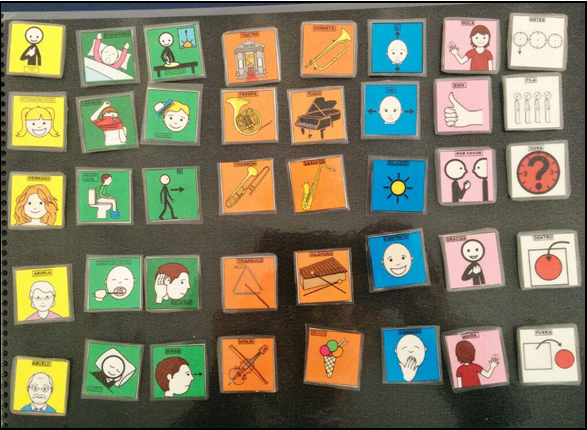
\includegraphics[width=0.7\linewidth]{Imagenes/Bitmap/tablerofisico}
	\caption{Tablero pictográfico en el que el usuario señala lo que quiere comunicar.}
	\label{fig:tablerofisico}
\end{figure}




Un ejemplo de ello son los TFGs de Pictar y PicTableros, ambos son herramientas online basadas en pictogramas y tableros respectivamente. Por ello tendremos como referencia estas herramientas en el desarrollo de nuestro TFG ya que tienen implementadas características con las que nos podremos apoyar como por ejemplo traducción de un texto a pictogramas, búsqueda de pictogramas y editor de tablero.\\

\textcolor{blue} {NO TENEMOS MUY CLARO ESTE PARRAFO \\
	Durante este tiempo, además de estas herramientas, han surgido muchas más, cada una con sus características y funcionalidades únicas. Pero al final queda la sensación que nunca se podía hacer\textbf{ todo en un mismo lugar}, y lo que le falta a una lo tiene otra herramienta, etc.}

Por lo mencionado, existe una necesidad de crear una herramienta que unifique las mejores características de cada herramienta y permita crear y editar tableros en un mismo lugar con la mayor facilidad posible. Afortunadamente, ya existe una base con la que nos podemos apoyar, gracias a proyectos de años anteriores como hemos mencionado, con ideas que se quedaron como trabajo futuro y algunas más que pueden ser de mucha utilidad. \textcolor{blue}{¿Hace falta que expliquemos aquí lo que queremos hacer?}



\section{Objetivos}
\label{cap1:sec:Objetivos}

Teniendo en cuenta las metas descritas anteriormente que se quieren conseguir podemos destacar los siguientes objetivos:
\begin{itemize}
\item Diseñar una aplicación web que permita la edición de tableros, búsquedas de pictogramas y traducción de texto a pictogramas. 

\item Afianzar conocimientos adquiridos durante la carrera y explorar nuevas tecnologías que nos ayuden en la realización del TFG.
\end{itemize}	
Para el primer objetivo se utilizarán aplicaciones de referencia como Pictar y PicTableros ya que incluyen herramientas que necesitaremos pero que mejoraremos su funcionalidad. Se pretende crear una aplicación web multiplataforma sencilla y fácil de utilizar para personas con trastorno del espectro autista. 


\section{Estructura de la memoria}
\label{cap1:sec:Estructura}

La estructura para memoria se encuentra dividida en [x] capítulos, a continuación se explicará brevemente su contenido.
\begin{itemize}
	\item En los capítulos 1 y 2, se expondrá el contexto bajo el cual se ha realizado el trabajo junto a la motivación y objetivos para realizarlo. El capítulo 1 está escrito en español y el 2 en inglés \textcolor{blue}{Esto no se si tiene mucho sentido, pues ya te has leído el capítulo 1 o 2...}
	\item En el capítulo 3 se explicará qué es un pictograma y los distintos sistemas de comunicación con ellos. Además se analizarán las distintas herramientas relacionadas con pictogramas haciendo énfasis en la edición de tableros.
\end{itemize}	




